% !TeX program = xelatex
% !TeX encoding = UTF-8
\documentclass[UTF8,zihao=-4,a4paper]{ctexart}

\usepackage[a4paper,top=2.35cm,bottom=2.35cm,left=2.55cm,right=2.55cm,headheight=15pt]{geometry}
\usepackage{booktabs}
\usepackage{tabularx}
\usepackage{longtable}
\usepackage{array}
\usepackage{amsmath}
\usepackage{enumitem}
\usepackage{xcolor}
\usepackage{listings}
\usepackage{graphicx}
\usepackage{tikz}
\usetikzlibrary{arrows.meta,positioning,shapes.geometric}
\usepackage{fancyhdr}
\usepackage{hyperref}
\usepackage{url}

\definecolor{Navy}{HTML}{17365D}
\definecolor{LightBlue}{HTML}{EAF2F8}
\definecolor{SoftGray}{HTML}{F5F6F7}
\definecolor{CodeGreen}{HTML}{2E7D32}
\definecolor{CodeRed}{HTML}{A33A2B}

\hypersetup{
  colorlinks=true,
  linkcolor=Navy,
  urlcolor=Navy,
  citecolor=Navy,
  pdftitle={软件测试综合实验报告：校园出行天气风险分析工具},
  pdfauthor={学生信息待填写}
}

\pagestyle{fancy}
\fancyhf{}
\fancyhead[L]{软件测试综合实验报告}
\fancyhead[R]{校园出行天气风险分析工具}
\fancyfoot[C]{\thepage}

\setlength{\parindent}{2em}
\setlength{\parskip}{0.25em}
\setlength{\emergencystretch}{3em}
\setlist{nosep,leftmargin=2.2em}
\renewcommand{\arraystretch}{1.3}

\lstdefinestyle{pythonstyle}{
  language=Python,
  basicstyle=\ttfamily\footnotesize,
  keywordstyle=\color{Navy}\bfseries,
  stringstyle=\color{CodeGreen},
  commentstyle=\color{gray},
  backgroundcolor=\color{SoftGray},
  frame=single,
  rulecolor=\color{gray!35},
  breaklines=true,
  showstringspaces=false,
  numbers=left,
  numberstyle=\tiny\color{gray},
  xleftmargin=1.6em,
  framexleftmargin=1.0em
}
\lstdefinestyle{shellstyle}{
  basicstyle=\ttfamily\footnotesize,
  backgroundcolor=\color{SoftGray},
  frame=single,
  rulecolor=\color{gray!35},
  breaklines=true,
  showstringspaces=false
}

\newcommand{\code}[1]{\texttt{#1}}
\newcommand{\risk}[1]{\textcolor{CodeRed}{\textbf{#1}}}
\newcommand{\blankfield}[1]{\underline{\hspace{#1}}}

\begin{document}

\begin{titlepage}
\thispagestyle{empty}
\begin{center}
\vspace*{1.5cm}
{\heiti\zihao{-1} 软件测试综合实验报告}\par
\vspace{1.2cm}
{\heiti\zihao{2} 校园出行天气风险分析工具}\par
\vspace{0.5cm}
{\zihao{3} 服务单元测试、持续集成测试与程序性能跟踪}\par

\vfill
\renewcommand{\arraystretch}{1.8}
\begin{tabular}{rl}
课程名称：& 软件测试实验 \\
姓\qquad 名：& \blankfield{5.5cm} \\
学\qquad 号：& \blankfield{5.5cm} \\
班\qquad 级：& \blankfield{5.5cm} \\
指导教师：& \blankfield{5.5cm} \\
\end{tabular}

\vfill
{\zihao{4} 实验日期：2026年8月19日}\par
{\zihao{4} 报告日期：2026年8月19日}\par
\vspace{1cm}
\end{center}
\end{titlepage}

\begin{abstract}
本文以 Python“校园出行天气风险分析工具”为统一对象，完成三个软件测试实验。实验一针对 Open-Meteo 地理编码与天气预报 REST API，先分析输入、HTTP、JSON 契约、动态数据与本地业务规则风险，再设计离线单元测试和真实接口测试；24 项离线测试与 7 项网络测试全部通过。实验二使用 GitHub Actions 配置自动安装、分层测试、JUnit 报告、wheel/源码包构建和制品上传；本地复演中 39 项测试及两个分发包校验通过，真实云端运行 32258964845 又完成 32 项离线测试和 7 项接口测试，JUnit 均为零失败、零错误，并成功上传测试报告和分发包。实验三使用固定的 24 小时数据，以 cProfile 和 tracemalloc 分析 240,000 个事件的批处理；定位到重复日期解析、重复排序与大中间列表，优化后在功能结果相同的条件下，跟踪时间减少 39.90\%，Python 分配峰值从 21,573,080 B 降至 2,840 B。实验强调风险驱动、测试分层、证据可追溯与结论边界。

\noindent\textbf{关键词：}REST API；pytest；持续集成；GitHub Actions；cProfile；tracemalloc
\end{abstract}

\clearpage
\tableofcontents
\clearpage

\section{实验总体设计}

\subsection{选题与测试对象}

测试对象是一个精简的校园出行天气风险分析工具。用户输入城市名后，程序调用 Open-Meteo 地理编码 API 获得经纬度，再调用天气预报 API 获取逐小时温度、降水概率和风速，最后由本地确定性规则生成“高温”“低温”“建议带伞”“注意大风”或“适宜出行”等提示。

选择该对象的原因是：无需 API Key，便于复现；同时包含远程 HTTP/JSON 契约、实时动态数据、本地业务规则、自动打包和批处理性能等问题，可以让三个实验共享源码而保持清晰的测试边界。

\begin{center}
\begin{tikzpicture}[
  node distance=0.8cm and 0.75cm,
  box/.style={draw=Navy,rounded corners,fill=LightBlue,minimum height=0.85cm,text width=2.4cm,align=center},
  arrow/.style={-{Latex[length=2.5mm]},thick,color=Navy}
]
\node[box] (input) {城市名输入};
\node[box,right=of input] (geo) {地理编码 REST API};
\node[box,right=of geo] (forecast) {天气预报 REST API};
\node[box,below=of forecast] (rule) {本地风险规则};
\node[box,left=of rule] (ci) {pytest 与 CI};
\node[box,left=of ci] (profile) {固定数据性能跟踪};
\draw[arrow] (input) -- (geo);
\draw[arrow] (geo) -- (forecast);
\draw[arrow] (forecast) -- (rule);
\draw[arrow] (rule) -- (ci);
\draw[arrow] (ci) -- (profile);
\end{tikzpicture}
\end{center}

\subsection{三个实验的关系}

\begin{table}[htbp]
\centering
\caption{实验选择与核心证据}
\begin{tabularx}{\textwidth}{p{0.18\textwidth}p{0.31\textwidth}X}
\toprule
实验 & 核心问题 & 主要证据 \\
\midrule
服务单元测试 & 接口和业务规则在正常、边界、异常情况下是否满足约定 & pytest 日志、两份 JUnit、API 样例 \\
持续集成测试 & 修改后能否自动测试、打包并保存报告 & Actions YAML、本地复演日志、JUnit、wheel、sdist、哈希 \\
程序性能跟踪 & CPU 时间和对象分配花在哪里，改进是否保持正确且有效 & 等价性测试、两份 \code{.prof}、pstats 摘要、内存 JSON \\
\bottomrule
\end{tabularx}
\end{table}

项目使用 Python 3.13.7 和 pytest 8.4.1；第三方库保存在项目内 \code{.local-packages}，生成报告、缓存、构建输出与本地依赖均由 \code{.gitignore} 排除。源码采用 \code{src/} 布局，HTTP 请求设置超时，并把底层错误转换为项目异常。

\section{实验一：服务单元测试}

\subsection{接口介绍与风险分析}

地理编码端点按城市名搜索位置，返回名称、国家代码、纬度和经度；天气预报端点按经纬度、天数、时区和小时变量返回数组。测试不把 HTTP 200 当作充分条件，而是继续验证 JSON 可解码、字段类型、数组对齐、单位、范围和业务不变量。Open-Meteo 官方文档提供了两个端点的参数和返回结构\cite{openmeteo-geocoding,openmeteo-forecast}。

\begin{longtable}{p{0.21\textwidth}p{0.27\textwidth}p{0.41\textwidth}}
\toprule
风险 & 缺陷表现 & 测试策略 \\
\midrule
\endhead
非法本地输入 & 空城市名、坐标或天数越界仍发送请求 & 参数化边界测试，要求在网络前抛出明确异常 \\
HTTP/网络失败 & 超时、非 2xx 被误作正常 JSON & 模拟底层请求失败并检查 \code{WeatherServiceError} \\
JSON 与契约损坏 & 非 JSON、缺字段、小时数组长度不一致 & 伪响应单元测试与契约断言 \\
实时数据变化 & 精确天气值导致测试偶发失败 & 只断言结构、单位、范围、时区与数组不变量 \\
业务规则错误 & 高温、低温、降水和风速阈值误判 & 对纯函数 \code{assess\_hour} 进行参数化测试 \\
第三方服务波动 & 网络问题误判成本地回归 & 离线测试与 \code{network} 标记测试分开执行 \\
\bottomrule
\end{longtable}

\subsection{测试设计与关键实现}

HTTP 访问封装在 \code{OpenMeteoClient} 中，并通过可替换的 opener 注入测试替身。这样可在无网络条件下精确构造正常 JSON、HTTP 错误、非 JSON 和字段缺失。风险规则是纯函数，使用参数化表表达输入与期望标签：

\begin{lstlisting}[style=pythonstyle]
@pytest.mark.parametrize(
    ("temperature", "rain", "wind", "expected"),
    [
        (25, 10, 5, ["适宜出行"]),
        (36, 10, 5, ["高温"]),
        (-1, 80, 5, ["低温", "建议带伞"]),
        (25, 80, 45, ["建议带伞", "注意大风"]),
    ],
)
def test_assess_hour_is_parameterized(
    temperature, rain, wind, expected
):
    assert assess_hour(temperature, rain, wind) == expected
\end{lstlisting}

真实接口测试覆盖南京、北京和上海的地理编码，未知城市空结果，1/2 天数组长度，以及时区与单位。测试不依赖某一时刻的具体天气数值。

\subsection{执行结果}

2026年8月19日执行 \code{scripts/run-experiment-1.ps1}，证据目录为：

\begin{lstlisting}[style=shellstyle]
reports/experiment-1/20260819-114835/

Offline JUnit: tests=24, failures=0, errors=0, time=0.116s
Live API JUnit: tests=7, failures=0, errors=0, time=8.401s
API sample exit code: 0
\end{lstlisting}

真实样例定位到南京（32.06167, 118.77778），返回时区 \code{Asia/Shanghai}、UTC 偏移 28,800 秒，以及温度、降水概率和风速单位。样例只保存前三小时，既能作为响应结构证据，又避免把整份实时结果塞入报告。

\subsection{服务接口测试与类/函数单元测试比较}

两者都需要明确输入、执行、断言和隔离失败原因，也都能使用参数化和自动化框架。差别在于服务测试跨越 HTTP、序列化、网络和第三方系统，结果可能动态变化，速度慢且失败来源多；函数单元测试在本进程中运行，输入可控、结果稳定、定位更直接。因此本项目以大量快速离线测试作为基础，再用少量真实接口测试验证外部契约。

\section{实验二：持续集成测试}

\subsection{风险驱动的流水线设计}

持续集成的主要风险不是“没有 YAML 文件”，而是步骤遗漏、依赖漂移、网络测试与本地测试混淆、测试通过但包内容缺失、运行证据丢失。因此工作流按以下顺序设计：

\begin{enumerate}
  \item 在推送、拉取请求和手动触发时启动 Ubuntu Runner；
  \item 检出源码，安装 Python 3.13 和锁定的开发依赖；
  \item 先执行离线测试并生成 \code{junit-offline.xml}；
  \item 单独执行真实 API 测试并生成 \code{junit-network.xml}；
  \item 用 PyPA build 构建 wheel 与源码包；
  \item 无论测试是否失败都尽量上传报告；成功构建后上传分发包。
\end{enumerate}

GitHub 官方 Python CI 文档给出了 \code{setup-python}、pytest、构建和 artifact 的常见组合\cite{github-python-ci}；工作流制品由 \code{upload-artifact@v4} 保存\cite{github-artifact}。

\subsection{关键配置}

\begin{lstlisting}[style=shellstyle]
name: Python CI
on: [push, pull_request, workflow_dispatch]

jobs:
  test-and-build:
    runs-on: ubuntu-latest
    steps:
      - uses: actions/checkout@v6
      - uses: actions/setup-python@v5
      - run: python -m pytest -m "not network" --junitxml=...
      - run: python -m pytest -m "network" --junitxml=...
      - run: python -m build
      - uses: actions/upload-artifact@v4
\end{lstlisting}

此外，\code{test\_project\_configuration.py} 检查工作流是否仍含测试、JUnit、构建和制品步骤；\code{verify\_distribution.py} 打开 wheel 与 sdist，确认客户端和风险模块确实进入包中。这避免只看构建命令退出码。

\subsection{本地复演与真实云端结果}

2026年8月19日执行 \code{scripts/run-experiment-2.ps1}，保存环境、测试、JUnit、构建、包校验和哈希。结果目录：

\begin{lstlisting}[style=shellstyle]
reports/experiment-2/20260819-175707/

JUnit: tests=39, failures=0, errors=0, skipped=0
Test time: 8.397 s
Build exit code: 0
Distribution verification exit code: 0
wheel: campus_weather_lab-0.1.0-py3-none-any.whl
sdist: campus_weather_lab-0.1.0.tar.gz
\end{lstlisting}

两个分发包均生成成功并通过内容检查，\code{artifacts.txt} 记录大小和 SHA-256。新增的 8 项离线检查使当前离线测试达到 32 项；加上 7 项真实接口测试，本地流水线共执行 39 项。

\begin{center}
\fcolorbox{CodeGreen}{green!4}{\parbox{0.91\textwidth}{
\textbf{云端证据状态：已完成。}提交 \code{a36b2f4} 推送到公开仓库后触发 GitHub Actions 运行 32258964845。作业 \code{test-and-build} 的检出、Python 环境、依赖安装、离线测试、真实接口测试、构建和两次制品上传步骤全部为 success。运行页：
\url{https://github.com/diydashi/campus-weather-lab/actions/runs/32258964845}
}}
\end{center}

云端 \code{pytest-reports} 已实际下载并解析：离线 JUnit 为 32 tests、0 failures、0 errors、0 skipped、0.148 s；接口 JUnit 为 7 tests、0 failures、0 errors、0 skipped、4.725 s。\code{python-distributions} 中存在 wheel 与 sdist；两个 artifact ZIP 分别为 1,479 B 和 38,182 B。运行从北京时间 21:35:31 开始，于 21:36:00 完成。

\begin{figure}[htbp]
  \centering
  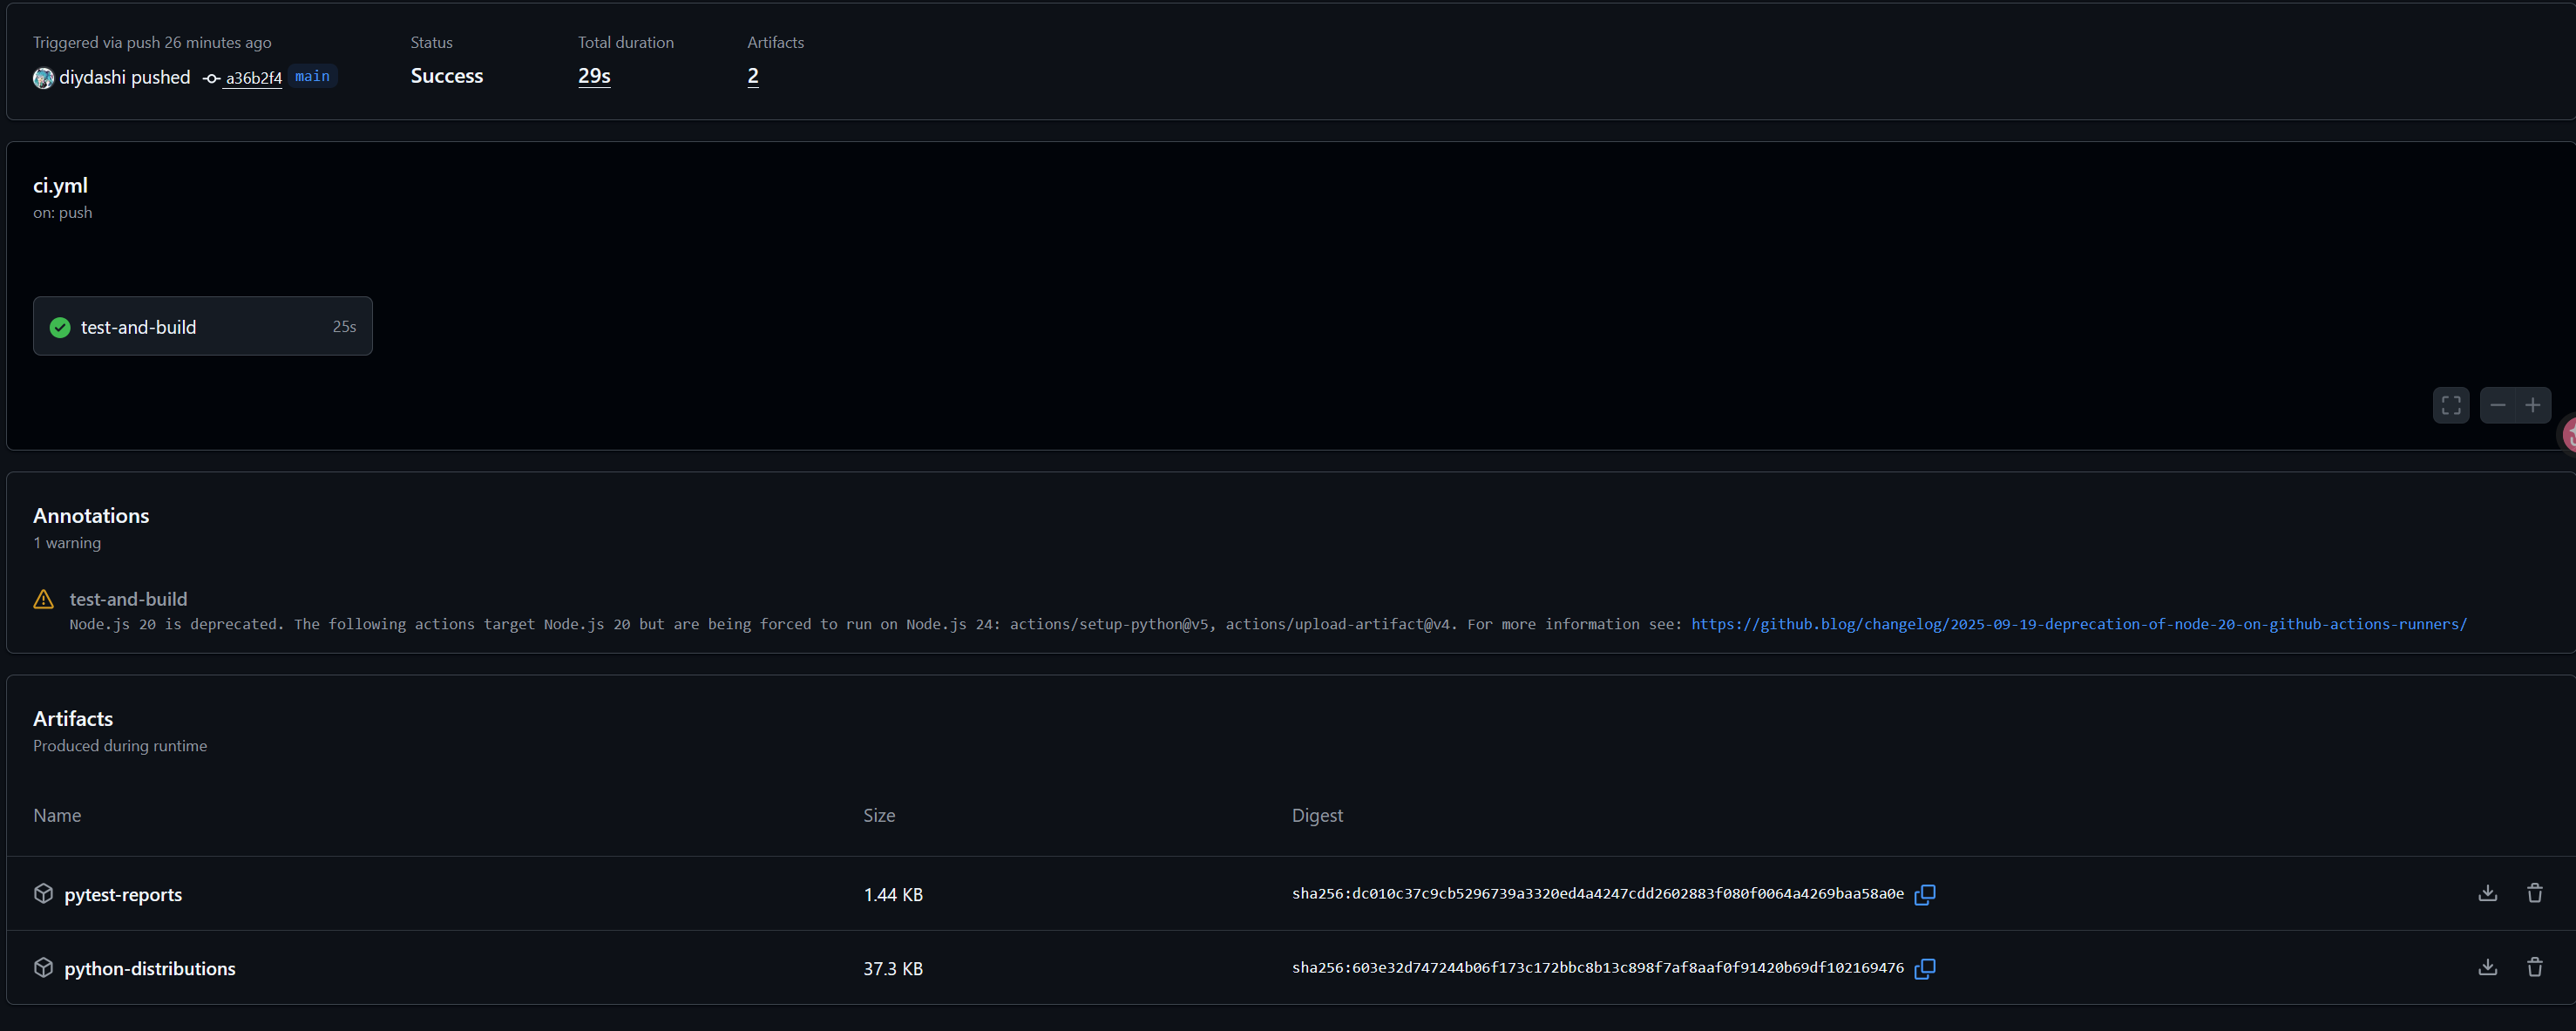
\includegraphics[width=0.96\textwidth,height=0.40\textheight,keepaspectratio]{images/github-actions-run.png}
  \caption{GitHub Actions 运行 32258964845 的真实成功页面}
  \label{fig:github-actions-evidence}
\end{figure}

图~\ref{fig:github-actions-evidence} 同时保留绿色作业和两个制品。页面中的黄色 Annotations 是 GitHub 对相关 Action 所用 Node.js 版本迁移的提醒，不代表测试失败；作业与整次运行的结论仍为 success。

\section{实验三：程序性能跟踪}

\subsection{工具选择与工作负载}

CPU 使用标准库 \code{cProfile} 和 \code{pstats}，优点是调用次数、自身时间和累计时间完整且可保存原始 \code{.prof}；内存使用 \code{tracemalloc}，读取 Python 分配的当前和峰值大小\cite{python-profile,python-tracemalloc}。与采样型 py-spy、行级 memory\_profiler 相比，标准库工具安装成本最低，适合本次小型、确定性本地工作负载；代价是存在跟踪开销，且 tracemalloc 不等于进程 RSS。

为排除网络干扰，输入固定为 24 条小时天气记录。运行 10,000 轮，共处理 240,000 个事件。基线版本每轮重新解析时间、排序并把所有结果加入大列表；优化版本只预处理一次，并用三个累计值代替大列表。

\subsection{正确性门禁}

优化前后必须保持相同业务结果。pytest 先以小轮数参数化比较，正式比较脚本再要求三个汇总字段完全相同：

\begin{table}[htbp]
\centering
\caption{优化前后功能结果}
\begin{tabular}{lrr}
\toprule
字段 & 基线 & 优化后 \\
\midrule
event\_count & 240,000 & 240,000 \\
time\_checksum & 165,600,000 & 165,600,000 \\
risk\_score & 620,000 & 620,000 \\
\bottomrule
\end{tabular}
\end{table}

\subsection{CPU 瓶颈与改进效果}

基线 cProfile 共记录 2,875,977 次调用，工作负载累计约 0.478 秒。主要热点为 \code{sum}、\code{\_risk\_score}、\code{sorted}、\code{assess\_hour}、排序 lambda 和 \code{datetime.fromisoformat}；日期解析被调用 480,000 次，说明同一数据在热循环中重复转换。

优化后总调用数为 1,426,022，工作负载累计约 0.245 秒。风险规则仍对每个事件执行，是合理热点；重复解析和排序基本移出热循环。原始证据保存在两个 \code{.prof} 及按累计时间排序的文本统计中。

\subsection{内存和同步计时结果}

\begin{table}[htbp]
\centering
\caption{相同 tracemalloc 条件下的性能对照}
\begin{tabular}{lrrr}
\toprule
指标 & 基线 & 优化后 & 变化 \\
\midrule
墙钟时间 & 0.7499 s & 0.4507 s & 减少 39.90\% \\
加速比 & \multicolumn{2}{c}{1.6639 倍} & --- \\
当前跟踪内存 & 112,452 B & 1,536 B & 明显下降 \\
Python 分配峰值 & 21,573,080 B & 2,840 B & 减少 99.9868\% \\
\bottomrule
\end{tabular}
\end{table}

内存差异来自对象生命周期：基线列表持有 240,000 个元组直到函数结束；优化版只保留 24 条预处理记录和少量整数。cProfile 的独立结果也显示约 0.478 秒降至 0.245 秒，因此时间改善并非只出现在内存跟踪计时中。

这些数字是本机单次证据，受系统负载、Python 版本和 profiler 开销影响。结论应表达为“在本次固定条件下明显改善，并且热点变化与代码改动相符”，不能把小数位推广为所有机器的绝对性能。

\section{问题、解决方法与个人分析}

\subsection{动态数据不能使用固定预言}

开始设计 API 测试时，最直观的做法是断言某个城市的具体温度，但实时天气必然变化。解决方法是把测试预言改为稳定不变量：数组长度、单位、时区、范围、国家代码和字段类型；具体数据只作为带时间戳的样例留证。这使测试既能发现契约变化，又不会每天随机失败。

\subsection{网络测试与本地缺陷容易混淆}

真实 API 失败可能来自网络和第三方服务。项目通过 pytest 标记把 32 项离线检查与 7 项真实接口测试分层，CI 也生成两份 JUnit。改进方向是给网络测试增加有限重试、定时监控和失败分类，但不应让重试掩盖持续的服务契约变化。

\subsection{本地复演与云端运行不能混写}

持续集成配置和核心命令先在 Windows 本地成功，但该事实本身不能证明 Ubuntu Runner、GitHub 事件上下文和 artifact 服务可用。因此初稿将云端状态写为待验证；远程仓库建立后才推送提交并记录运行 32258964845。随后又下载解析 JUnit、核对分发包名称，使结论从“本地可运行”升级为“托管流水线已真实闭环”。这比只放一个绿色图标更容易复核。

\subsection{优化容易破坏功能}

把大列表改成累计值有可能改变排序或汇总语义。因此在比较性能前先做等价性测试，并让比较脚本在结果不同的时候失败。该方法体现性能优化的基本原则：先守住正确性，再接受更快或更省内存的实现。

\subsection{可继续改进的方面}

\begin{itemize}
  \item CI 增加 Python 3.11--3.13 矩阵、安装后冒烟测试和分支保护；
  \item 性能实验重复多轮，报告中位数和四分位距，并用采样 profiler 与操作系统 RSS 交叉验证；
  \item API 测试增加响应模式版本记录与限流处理，避免第三方接口长期变化时只得到模糊失败；
  \item 最终提交前仅在本地补充姓名学号，避免公开仓库暴露完整个人信息。
\end{itemize}

\section{结论}

三个实验围绕同一 Python 项目形成连续验证：实验一从风险出发建立 24 项离线测试和 7 项真实接口测试；实验二把当前 39 项测试、JUnit、打包和制品保存组织成 GitHub Actions 工作流，完成本地复演后，又由真实托管运行 32258964845 验证测试、构建和制品上传；实验三用 CPU 与内存跟踪定位重复解析、重复排序和大列表，优化后在结果等价前提下获得明确改善。实验结果、环境、日志、机器可读报告、远程提交号和运行链接均已记录，三个实验的必备链路均已闭合。

\section*{大语言模型使用说明}
\addcontentsline{toc}{section}{大语言模型使用说明}

本实验使用大语言模型辅助分析课程 PDF、规划统一选题、建立代码和测试框架、补充测试证据、设计 CI 与性能工作负载，并协助编写 LaTeX 文档。主要 prompt 如下：

\begin{enumerate}
  \item “阅读分析综合实验2026.pdf，然后帮我规划一个容易实现、满足必备要求的实验方案。”
  \item “建立项目和 agents 指导文档，然后先进行实验一的实现和测试；第三方库尽量放在本地目录。”
  \item “完善实验一结果测试和记录；每个实验建立中文 LaTeX 学习说明，详细解释原理、方法和结果。”
  \item “完成剩余两个实验，然后使用 LaTeX 编写报告。”
  \item “接入公开 GitHub 仓库，测试是否可用，补全缺失环节并完善报告和说明文档。”
\end{enumerate}

回答摘要：建议复用校园天气风险工具完成服务单元测试、持续集成和程序性能跟踪；实现分层 pytest、真实接口留证、GitHub Actions、本地 CI 复演、分发包校验、cProfile/tracemalloc 对照实验，并生成学习说明与本报告。远程仓库建立后，辅助核对推送权限、真实运行状态、JUnit 和 artifacts；所有结论均由实际命令、报告文件和 GitHub 运行 32258964845 核验。完整记录见项目 \code{AI\_USAGE.md}。

\begin{thebibliography}{9}
\bibitem{openmeteo-geocoding}
Open-Meteo. \emph{Geocoding API Documentation}.\\
\url{https://open-meteo.com/en/docs/geocoding-api}

\bibitem{openmeteo-forecast}
Open-Meteo. \emph{Weather Forecast API Documentation}.\\
\url{https://open-meteo.com/en/docs}

\bibitem{github-python-ci}
GitHub Docs. \emph{Building and testing Python}.\\
\url{https://docs.github.com/en/actions/tutorials/build-and-test-code/python}

\bibitem{github-artifact}
GitHub Docs. \emph{Storing and sharing data from a workflow}.\\
\url{https://docs.github.com/en/actions/tutorials/store-and-share-data}

\bibitem{python-profile}
Python Software Foundation. \emph{The Python Profilers}.\\
\url{https://docs.python.org/3/library/profile.html}

\bibitem{python-tracemalloc}
Python Software Foundation. \emph{tracemalloc --- Trace memory allocations}.\\
\url{https://docs.python.org/3/library/tracemalloc.html}
\end{thebibliography}

\appendix
\section{关键文件与复现命令}

{\small
\setlength{\tabcolsep}{4pt}
\begin{tabular}{p{0.25\textwidth}>{\raggedright\arraybackslash}p{0.65\textwidth}}
\toprule
内容 & 路径 \\
\midrule
REST 客户端与风险规则 & \path{src/campus_weather/client.py}；\path{src/campus_weather/risk.py} \\
pytest 测试 & \code{tests/} \\
GitHub Actions & \path{.github/workflows/ci.yml} \\
性能工作负载 & \path{benchmarks/profile_workload.py} \\
实验设计记录 & \path{docs/experiment-1.md} 至 \path{docs/experiment-3.md} \\
详细学习说明 & \code{说明文档/} 下三个实验子目录的 \code{main.tex} \\
大模型记录 & \code{AI\_USAGE.md} \\
\bottomrule
\end{tabular}
}

\begin{lstlisting}[style=shellstyle]
# 实验一：分层 API/单元测试并留证
powershell -File ./scripts/run-experiment-1.ps1

# 实验二：本地复演 CI、打包、校验并留证
powershell -File ./scripts/run-experiment-2.ps1

# 实验三：CPU/内存跟踪、等价比较并留证
powershell -File ./scripts/run-experiment-3.ps1
\end{lstlisting}

\end{document}
